\section{Xây dựng ứng dụng}

\subsection{Thư viện và công cụ sử dụng}

\begin{table}[H]
  \centering
  \renewcommand{\arraystretch}{1.2}
  \begin{tabular}{|l|p{5cm}|p{2.5cm}|p{5.5cm}|}
    \hline
    \textbf{STT} & \textbf{Mục đích}        & \textbf{Công cụ}           & \textbf{Địa chỉ URL}          \\
    \hline
    1            & Chỉnh sửa mã nguồn       & Visual Studio Code         & https://code.visualstudio.com \\
    \hline
    2            & Cơ sở dữ liệu            & MongoDB                    & https://www.mongodb.com       \\
    \hline
    3            & Kiểm thử API             & Postman                    & https://www.postman.com       \\
    \hline
    4            & Lưu trữ mã nguồn         & Github                     & https://github.com            \\
    \hline
    5            & Vẽ bảng biểu             & Drawio, Mermaid, Swimlanes &
    \begin{minipage}[t]{6.5cm}
      https://app.diagrams.net \\
      https://mermaid.js.org \\
      https://swimlanes.io
    \end{minipage}                                                                            \\
    \hline
    6            & Thiết kế wireframe       & Whimsical                  & https://whimsical.com         \\
    \hline
    7            & Biên dịch Smart Contract & Foundry                    & https://book.getfoundry.sh    \\
    \hline
    8            & Kiểm thử Smart Contract  & Foundry, Tenderly          &
    \begin{minipage}[t]{6.5cm}
      https://book.getfoundry.sh\\
      https://tenderly.com
    \end{minipage}                                                                            \\
    \hline
  \end{tabular}
  \caption{Bảng tổng hợp các công cụ được sử dụng trong đề tài}
  \label{tab:tools}
\end{table}

\subsection{Kết quả thực nghiệm}
Sau đây là các hình ảnh của thực tế của ứng dụng web đã được phát triển được
chạy trên trình duyệt Firefox (Windows 11). Với các thiết bị khác, giao diện sẽ
co giãn phù hợp với kích thước màn hình nhưng lượng thông tin không thay đổi
nhiều

\begin{figure}[H]
  \centering
  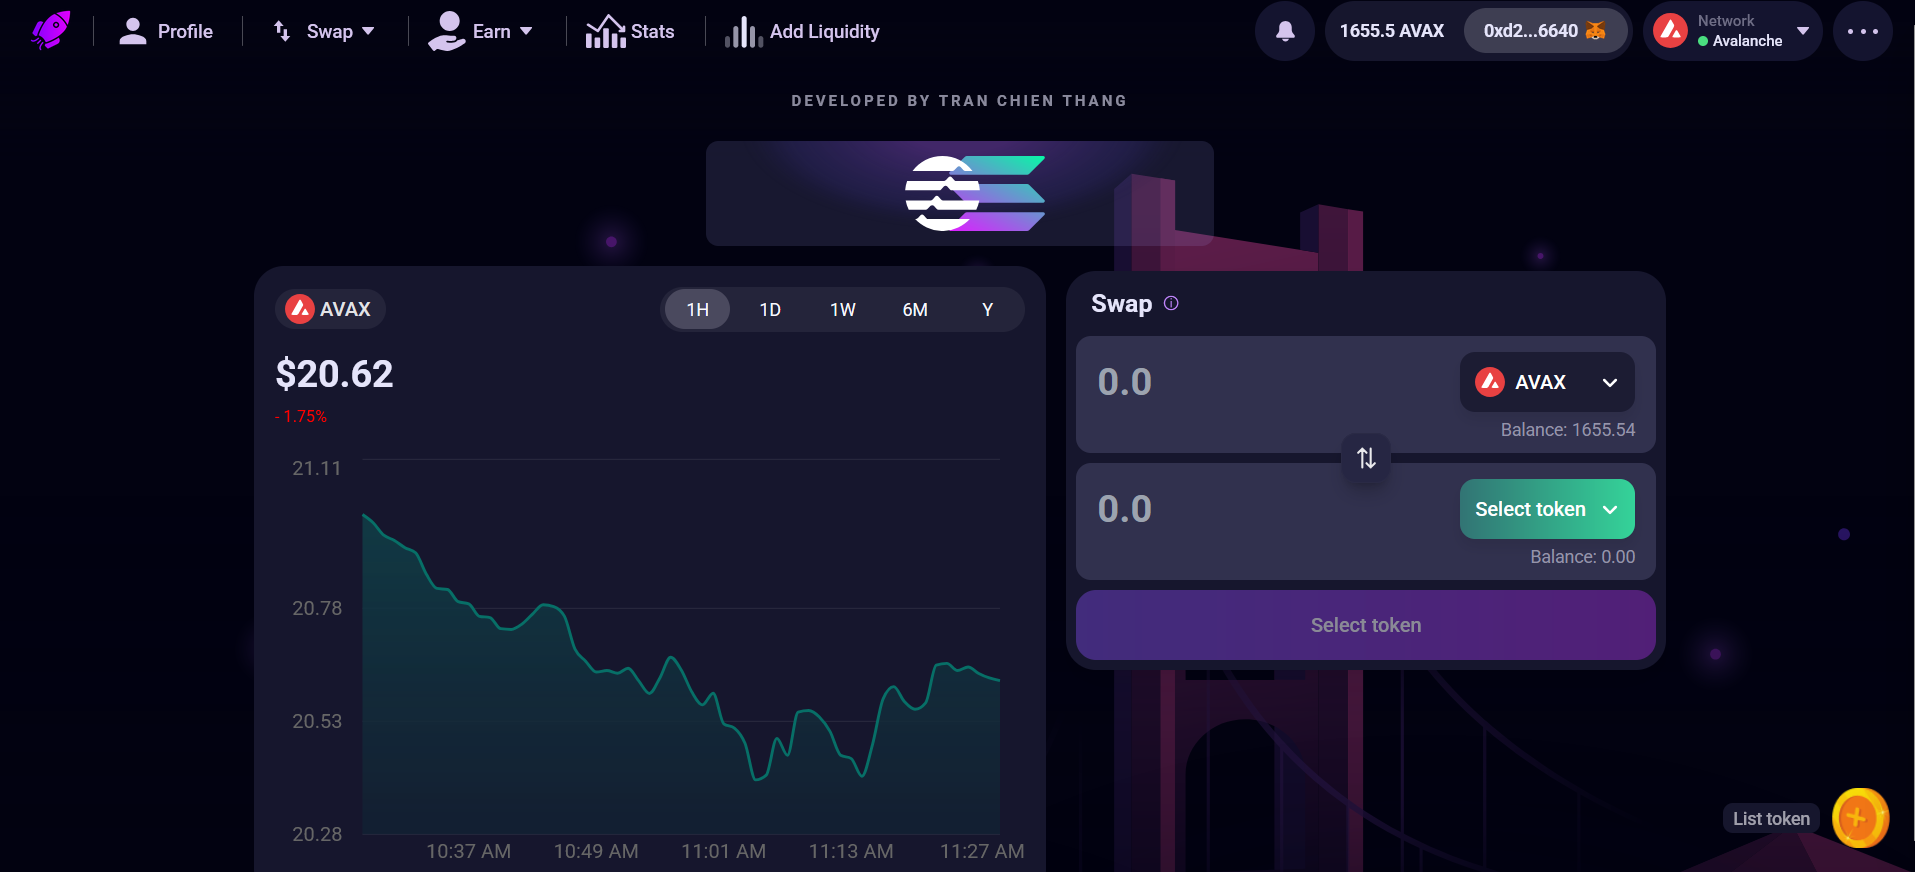
\includegraphics[width=1\textwidth]{figures/c3/MainScreenRel.png}
  \caption{Giao diện màn hình chính của ứng dụng.}
  \label{fig:architecture-diagram}
\end{figure}

\begin{figure}[H]
  \centering
  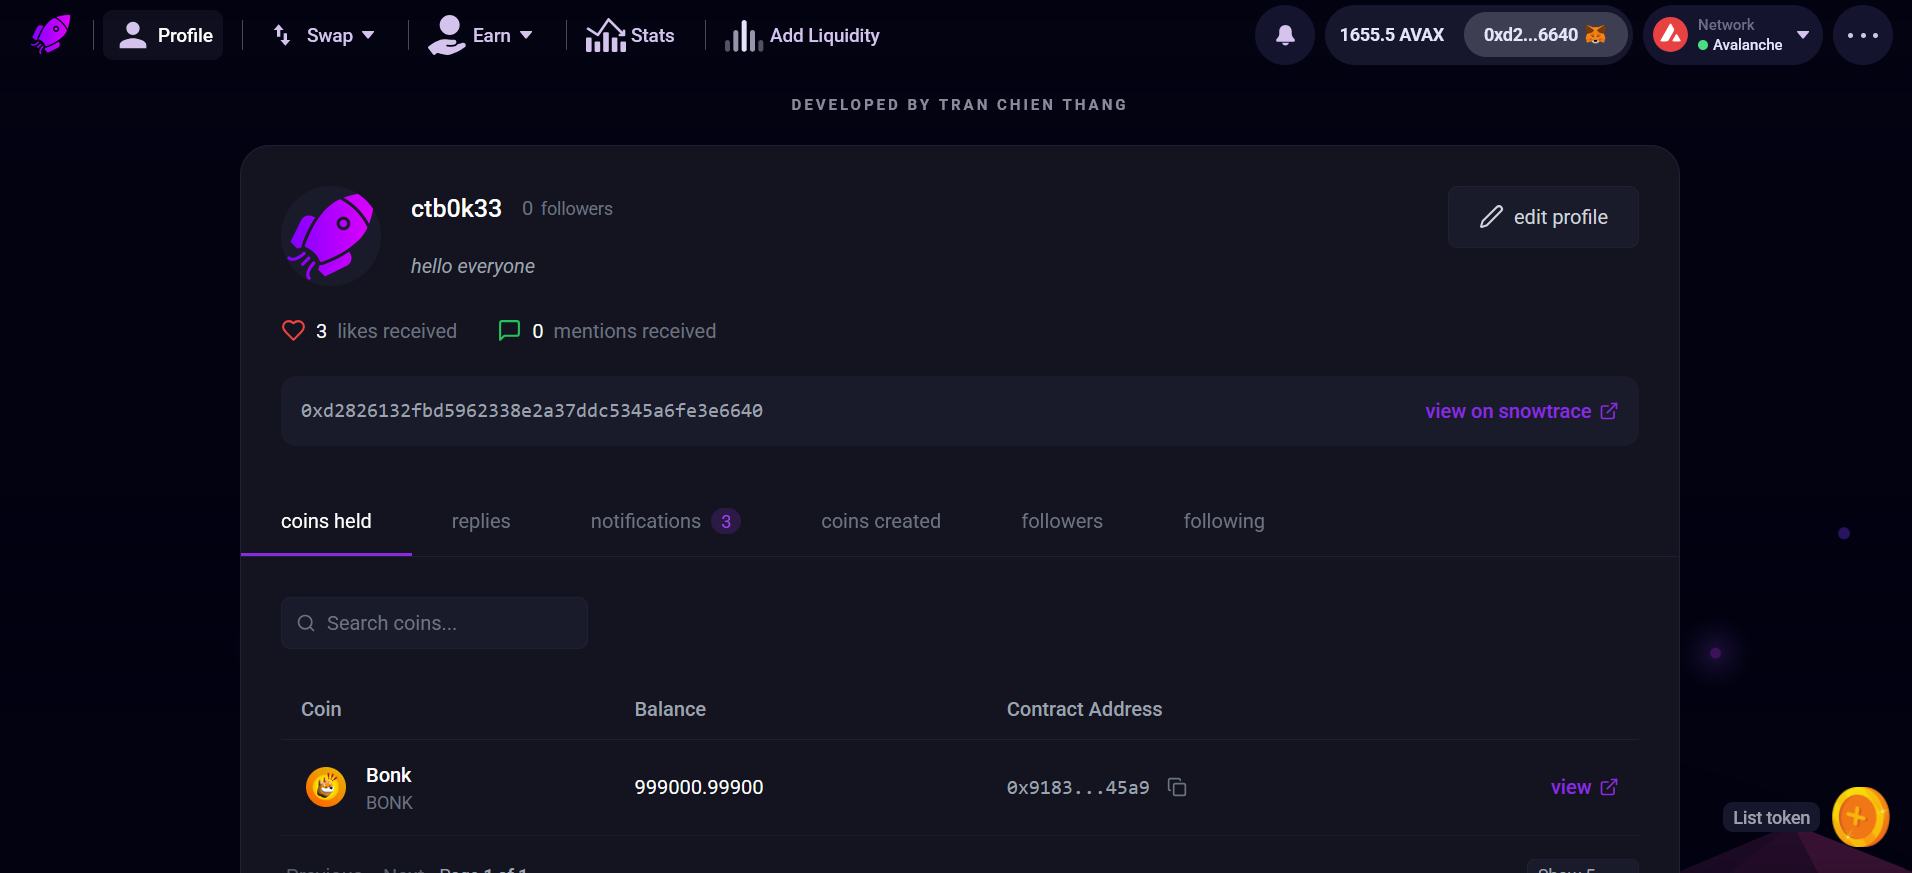
\includegraphics[width=1\textwidth]{figures/c3/UserProfileRel.png}
  \caption{Giao diện chức năng quản lý thông tin cá nhân.}
  \label{fig:architecture-diagram}
\end{figure}

\begin{figure}[H]
  \centering
  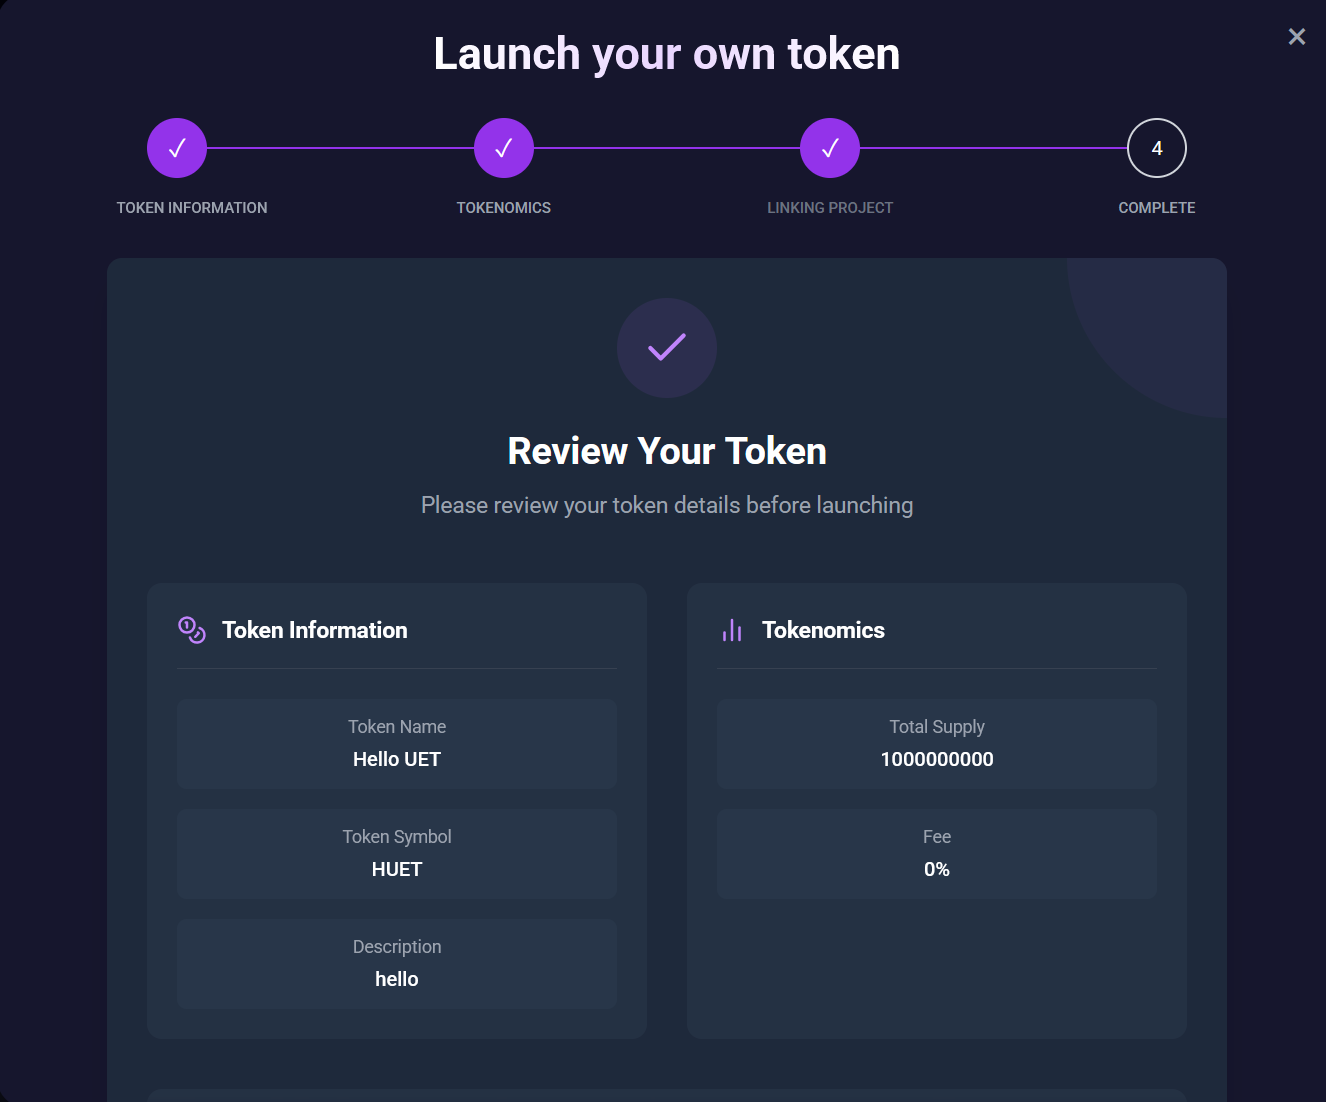
\includegraphics[width=1\textwidth]{figures/c3/CreateTokenRel.png}
  \caption{Giao diện chức năng tạo token mới.}
  \label{fig:architecture-diagram}
\end{figure}

\begin{figure}[H]
  \centering
  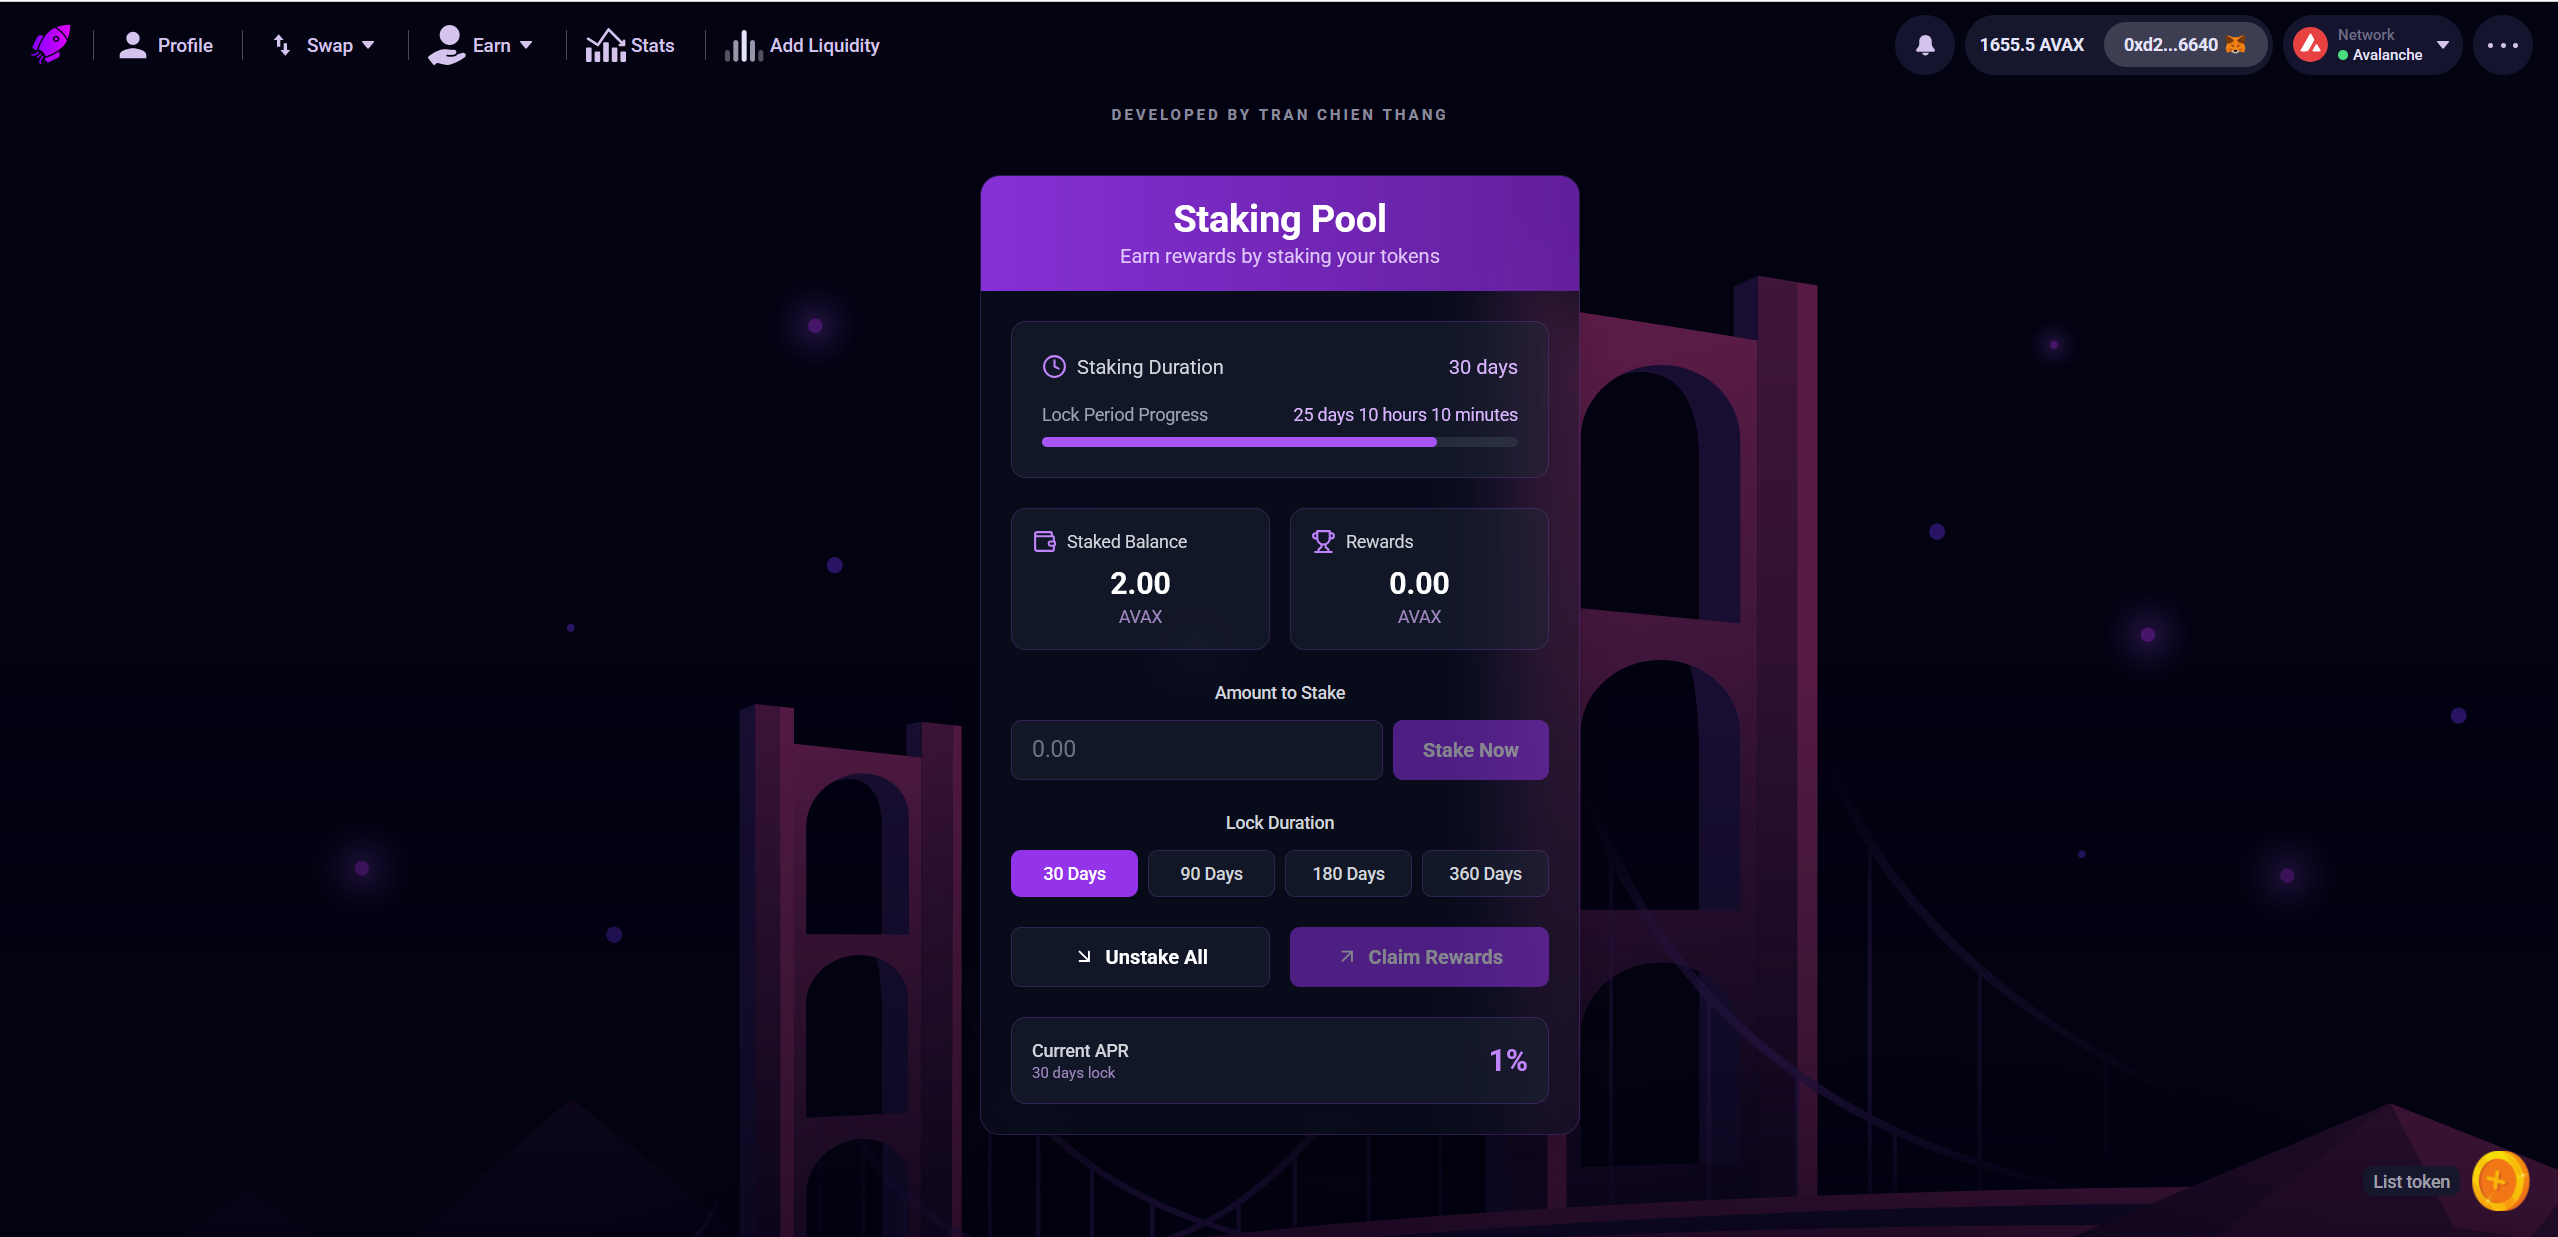
\includegraphics[width=1\textwidth]{figures/c3/StakingRel.png}
  \caption{Giao diện chức năng gửi tiết kiệm token.}
  \label{fig:architecture-diagram}
\end{figure}

\begin{figure}[H]
  \centering
  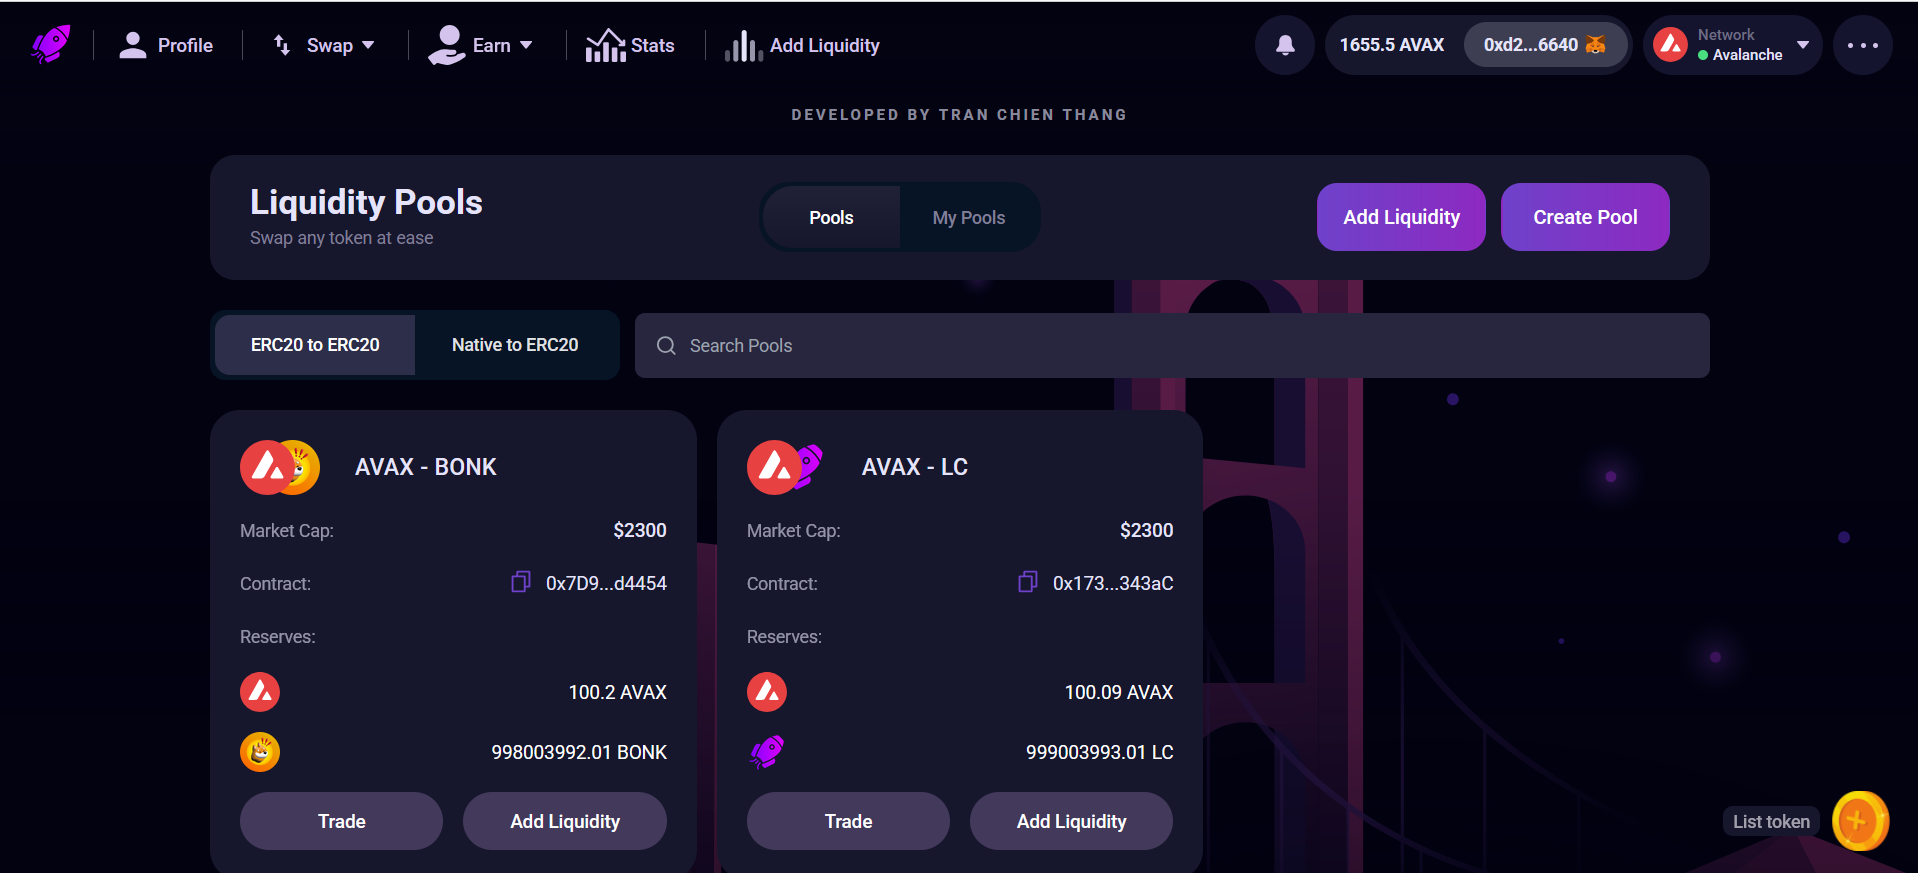
\includegraphics[width=1\textwidth]{figures/c3/SwapRel.png}
  \caption{Giao diện chức năng thao tác với các cặp giao dịch.}
  \label{fig:architecture-diagram}
\end{figure}

\begin{figure}[H]
  \centering
  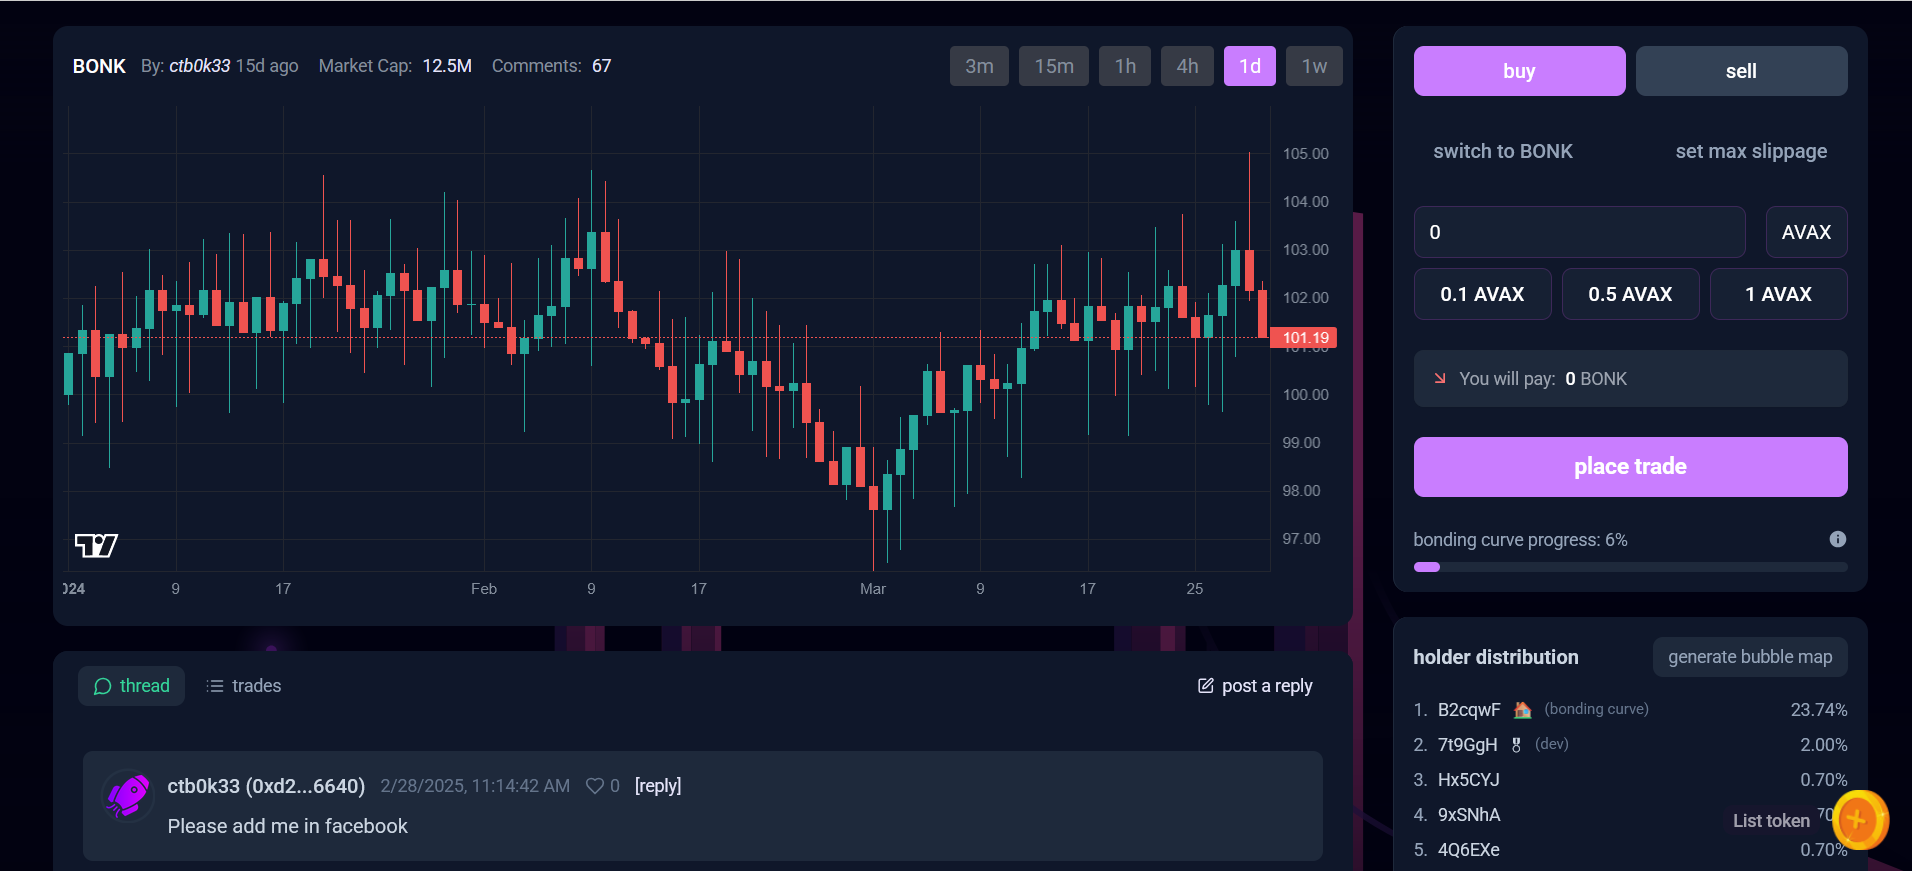
\includegraphics[width=1\textwidth]{figures/c3/TradeRel.png}
  \caption{Giao diện màn chức năng giao dịch token.}
  \label{fig:architecture-diagram}
\end{figure}

\begin{figure}[H]
  \centering
  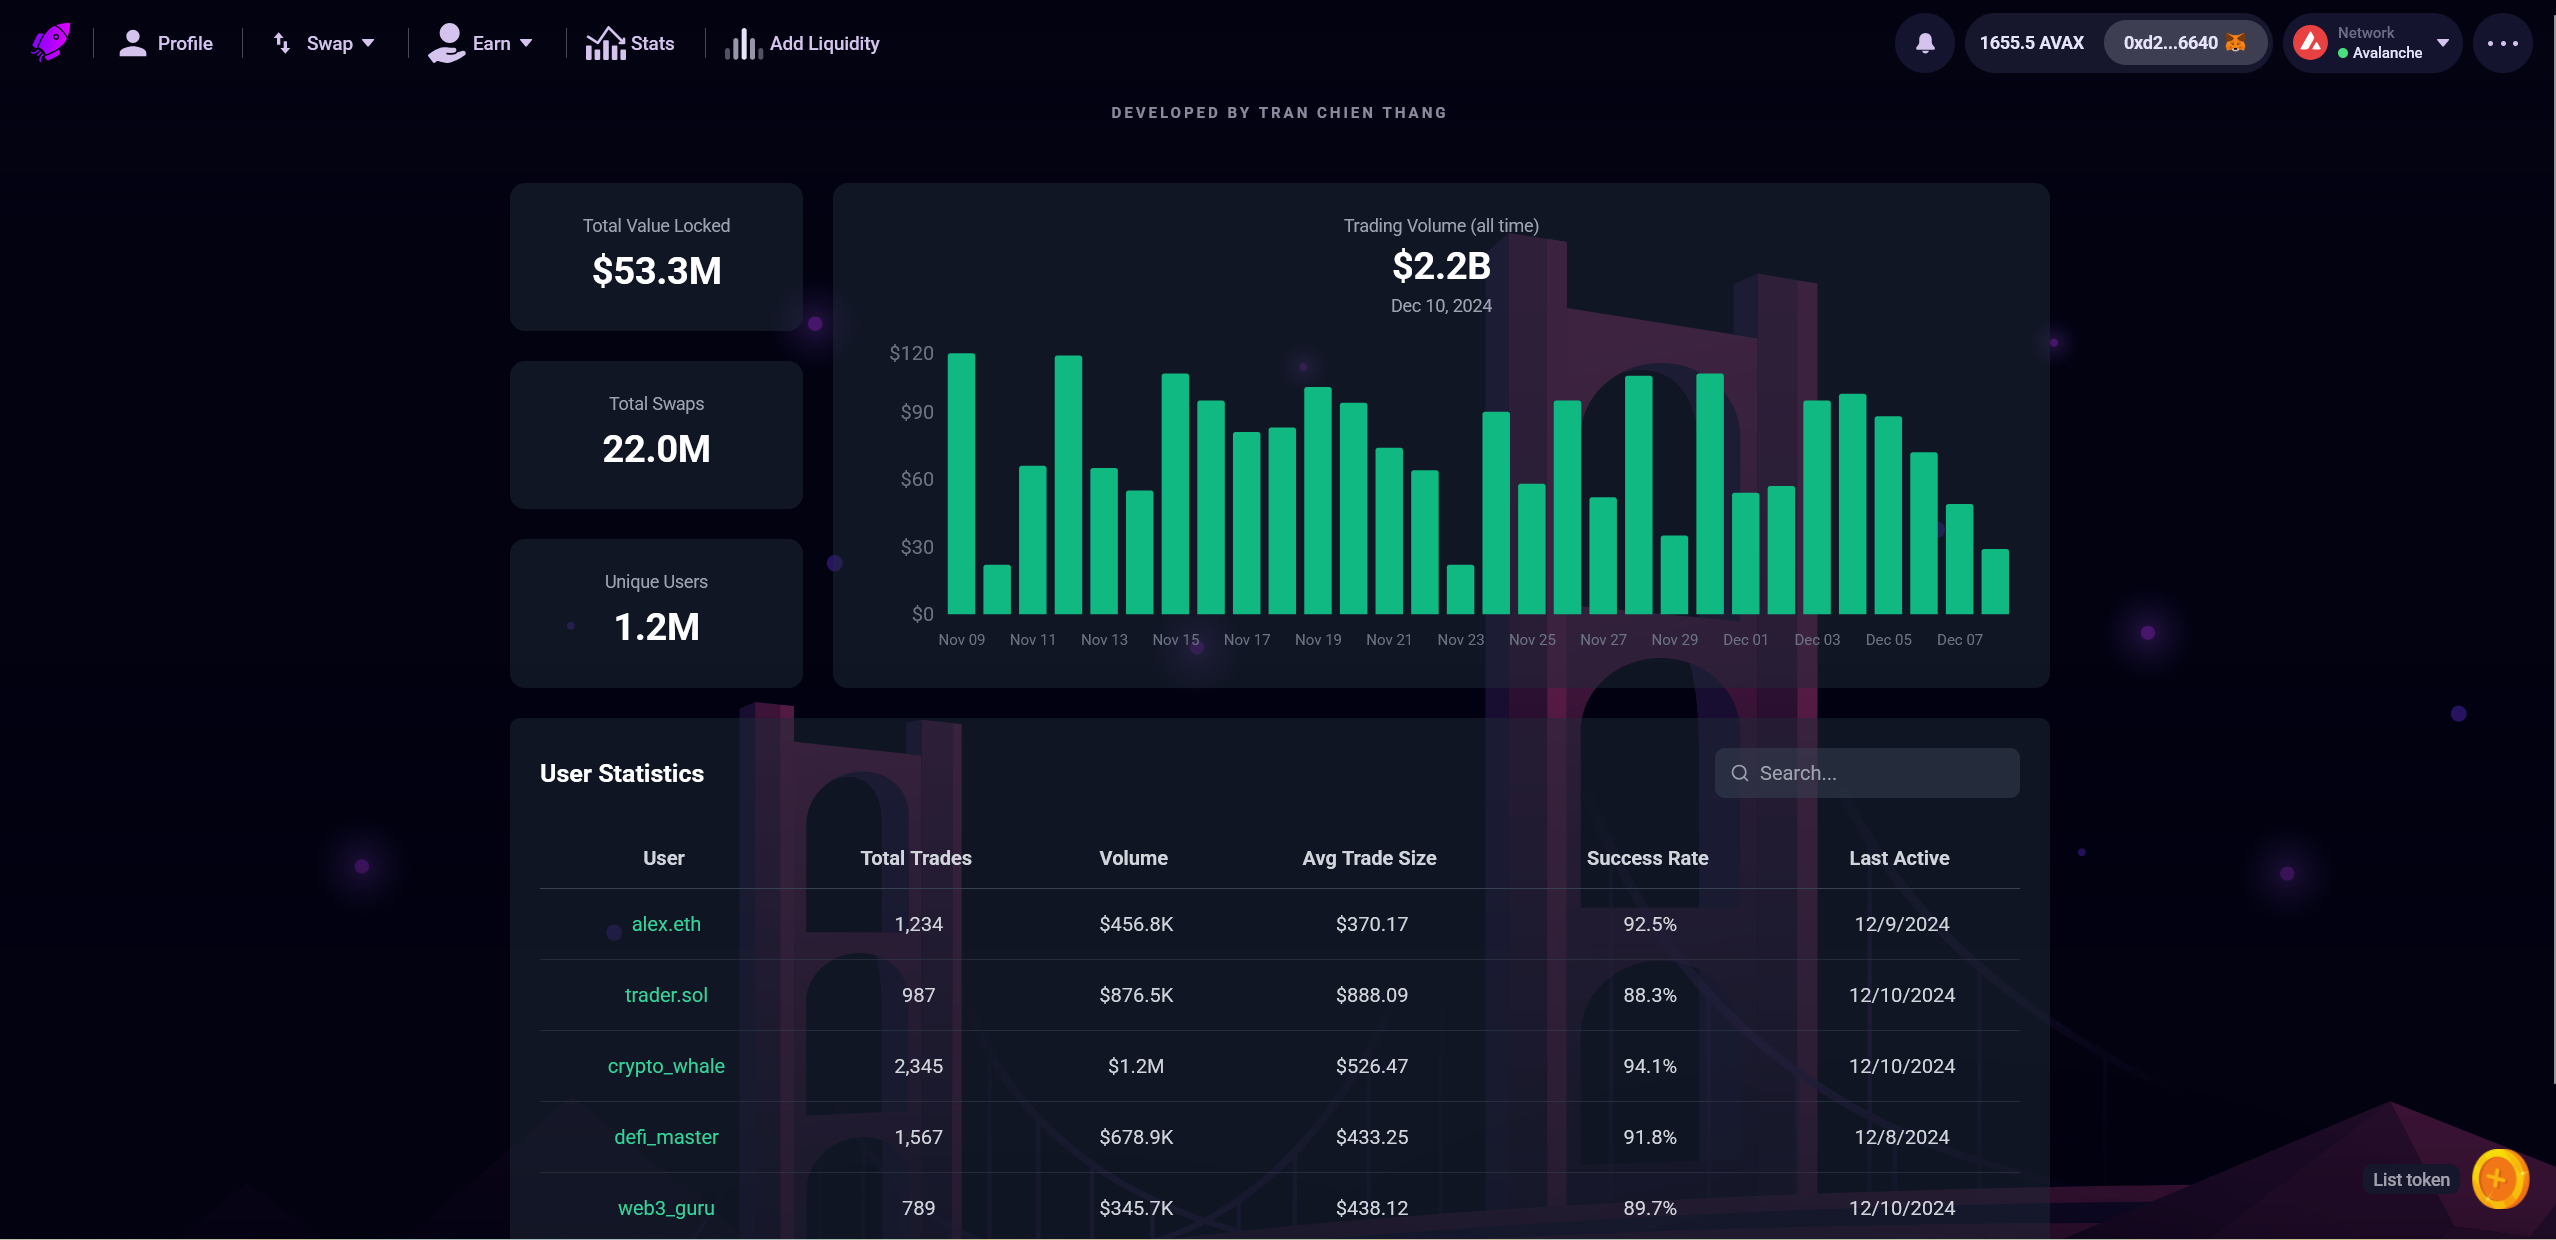
\includegraphics[width=1\textwidth]{figures/c3/StatsRel.png}
  \caption{Giao diện màn hình thống kê thông số của ứng dụng.}
  \label{fig:architecture-diagram}
\end{figure}

\section{Kiểm thử}
Khóa luận sẽ sử dụng các bộ test được sinh bởi hai kỹ thuật kiểm thử hộp đen là
phân hoạch tương đương và phân tích giá trị biên để thực hiện kiểm thử các chức
năng. Tại mỗi ca kiểm thử, khóa luận sẽ kiểm tra trạng thái trả về của API, kết
quả trả về từ hợp đồng thông minh. Thời gian phản hồi dưới 2 giây để thỏa mãn yêu
cầu phi chức năng tương ứng. Để thống nhất với quá trình phát triển, khóa
luận áp dụng kỹ thuật kiểm thử TDD (Test Driven Development). Theo đó, khóa
luận sẽ thiết kế các API, viết các bộ test tương ứng cho hợp đồng thông minh và thực
hiện việc phát triển
à kiểm thử song song. Quá trình kiểm thử sẽ được diễn ra tự động bằng cách sử
dụng ứng dụng POSTMAN cũng như thư viện foundry và tenderly trong quá trình
phát triển.
\clearpage
\begin{longtable}{|>{\raggedright\arraybackslash}p{3cm}|>{\raggedright\arraybackslash}p{5cm}|>{\raggedright\arraybackslash}p{5cm}|}
  \hline
  \textbf{Tính năng}                                                   & \textbf{Ngữ cảnh}                                                   & \textbf{Kết quả mong muốn} \\
  \hline
  Đăng nhập                                                            & 1) Kết nối ví metamask                                              &
  1) Giao diện thành công hiển thị địa chỉ ví và số dư của người dùng
  \newline
  2) Người dùng có thể sử dụng tất cả các tính năng còn lại của ứng dụng                                                                                                  \\
  \hline
  Quản lý tài khoản                                                    & 1) Người dùng xem thông tin tài khoản cá nhân.                      & 1) Hệ
  thống hiển thị chính xác thông tin các token người dùng đang sử hữu \newline 2)
  Hệ thống hiển thị chính xác tên, bio, ảnh đại diện của người dùng                                                                                                       \\
  \hline
  Cập nhật thông tin cá nhân                                           & 1) Người dùng cập nhật thông tin bio, ảnh đại diện
                                                                       & 1) Hệ thống thành công cập nhật thông tin cá nhân                                                \\
  \hline
  Tạo token                                                            & 1) Người dùng bấm vào "List token" \newline 2) Người dùng điền đầy
  đủ thông tin về token \newline 3) Người dùng chọn "confirm" và xác nhận giao
  dịch trên metamask                                                   & 1) Token được tạo thành công trên chuỗi khối \newline 2)
  Cặp giao dịch mới được tạo thành công trên chuỗi khối \newline 3) Token và cặp
  giao dịch mới hiển thị trên hệ thống với thông số chính xác                                                                                                             \\
  \hline

  Tạo token (số dư không đủ)                                           & Tương tự như ca kiểm thử "Tạo token"                                & 1) Hệ thống
  hiển thị thông báo tạo token thất bại                                                                                                                                   \\
  \hline

  Giao dịch token                                                      & 1) Người dùng bấm vào "Swap" \newline 2) Người dùng chọn cặp
  giao dịch mong muốn \newline 3) Người dùng chọn thực hiện giao dịch mua hoặc
  bán token                                                            & 1) Giao dịch thành công được ghi lại trên chuỗi khối \newline 2) Số
  dư trong ví của người dùng cập nhật thành công \newline 3) Thông tin về cặp
  giao dịch như số lượng token còn lại trong pool, giá token thay đổi chính xác.
  \newline 4) Thông tin giao dịch được ghi lại và hiển thị chính xác trên hệ
  thống                                                                                                                                                                   \\
  \hline

  Giao dịch token (số dư không đủ)                                     & Tương tự như ca kiểm thử "Giao dịch token"                          &
  1) Giao diện hiển thị giao dịch thất bại                                                                                                                                \\
  \hline

  Giao dịch token (Không đủ thanh khoản trong pool)                    & Tương tự như ca kiểm thử
  "Giao dịch token"                                                    & 1) Giao diện hiển thị thông báo "Not enough reserve in
  pool"                                                                                                                                                                   \\
  \hline

  Gửi tiết kiệm token                                                  & 1) Người dùng bấm vào "Earn", xong đó bấm vào "stake"
  \newline 2) Người dùng nhập số lượng token muốn gửi tiết kiệm và thời gian gửi
  tiết kiệm  \newline 3) Người dùng chọn "stake" và xác nhận giao dịch & 1) Giao
  dịch thành công được ghi lại trên chuỗi khối \newline 2) Số dư trong ví của
  người dùng cập nhật thành công \newline 3) Thông tin về stake của user hiển thị
  trên màn hình chính xác. \newline 4) Thông tin stake được ghi lại chính xác
  trên hệ thống                                                                                                                                                           \\
  \hline

  Gửi tiết kiệm token (chưa rút khoản gửi tiết kiệm cũ)                & Tương tự như ca kiểm
  thử "Gửi tiết kiệm token"                                            & 1) Giao diện hiển thị thông báo gửi tiết kiệm thất
  bại                                                                                                                                                                     \\
  \hline

  Gửi tiết kiệm token (số dư không đủ)                                 & Tương tự như ca kiểm thử "Gửi tiết kiệm
  token"                                                               & 1) Giao diện hiển thị thông báo gửi tiết kiệm thất bại                                           \\
  \hline

  Bình luận                                                            & 1) Người dùng bấm vào "Swap" \newline 2) Người dùng chọn cặp giao
  dịch mong muốn \newline 3) Người dùng để lại bình luận               & 1) Giao diện hiển thị
  bình luận thành công                                                                                                                                                    \\
  \hline

  Yêu thích bình luận                                                  & 1) Người dùng bấm vào "Swap" \newline 2) Người dùng chọn
  cặp giao dịch mong muốn \newline 3) Người dùng thích 1 bình luận của người dùng
  khác                                                                 & 1) Giao diện hiển thị ghi nhận thích bình luận thành công                                        \\
  \hline

  \caption{Các trường hợp kiểm thử.}
  \label{tab:account-management}
\end{longtable}

\begin{table}[htbp]
  \centering
  \begin{tabular}{|p{5cm}|c|c|}
    \hline
    \textbf{Tính năng kiểm thử} & \textbf{Kết quả} & \textbf{Chú thích}                 \\
    \hline
    Đăng nhập                   & Đạt              & Kiểm thử UI và API                 \\
    \hline
    Quản lý tài khoản           & Đạt              & Kiểm thử UI và API                 \\
    \hline
    Tạo token                   & Đạt              & Kiểm thử UI, API và Smart contract \\
    \hline
    Giao dịch token             & Đạt              & Kiểm thử UI, API và Smart contract \\
    \hline
    Gửi tiết kiệm token         & Đạt              & Kiểm thử UI, API và Smart contract \\
    \hline
    Rút tiết kiệm token         & Đạt              & Kiểm thử UI, API và Smart contract \\
    \hline
    Bình luận                   & Đạt              & Kiểm thử UI và API                 \\
    \hline
  \end{tabular}
  \caption{Kết quả kiểm thử chức năng}
  \label{tab:test-results}
\end{table}

\section{Đánh giá hiệu năng và phương hướng cải thiện của hệ thống}
Mặc dù các thử nghiệm đều chứng minh rằng hệ thống được phát triển thỏa mãn
và đáp ứng được tối thiểu các yêu cầu về chức năng và phi chức năng đã đặt ra.
Tuy nhiên, trong môi trường thực tế, sẽ cần nhiều sự cải thiện để hệ thống có
thể
hoạt động mượt mà và ổn định. Điều này vô cùng quan trọng vì khóa luận tập
trung phát triển một nền tảng cho phép người dùng giao dịch giữa các loại
token. Điều này sẽ góp phần làm giảm tối thiếu các giao dịch với độ trượt giá
cao, một điều rất quan trọng trong mọi hệ thống giao dịch.

Để nâng cao hiệu suất của hệ thống, khóa luận đặt ra các hướng
phát triển trong tương lai bao gồm: \textit{Áp dụng kỹ thuật caching, xây dựng
  dịch vụ worker riêng để quản lý giao dịch và phân bổ dịch vụ theo chiều rộng.}

Áp dụng hệ thống caching sẽ giúp cải thiện hiệu suất của hệ thống, đặc biệt với
những truy vấn offchain như lấy thông tin người dùng hay lấy thông tin về các
cặp giao dịch. Việc caching cũng làm giảm tải cho cơ sở dữ liệu, hạn chế các
truy vấn trực tiếp đến cơ sở dữ liệu chính. Việc lưu trữ dữ liệu trong bộ nhớ
cũng giảm dữ liệu cần truyền qua mạng, tăng tính sẵn sàng của dữ liệu trong hệ
thống.

Đối với mô đun giao dịch, việc xây dựng một dịch vụ worker riêng hoặc sử dụng worker từ các provider uy tín như
quicknode là cực kỳ quan trọng. Khi hệ thống mở rộng và số lượng các cặp giao
dịch tăng lên, việc truy vấn cơ sở dữ liệu về giao dịch liên tục để xây dựng mô
hình nến cho từng cặp giao dịch ở các timeframe khác nhau như khóa luận đang
triển khai là vô cùng tốn kém. Điều này sẽ có thể gây ra các vấn đề tiềm ẩn về
hiệu năng của hệ thống khi số lượng cặp giao dịch tăng cao.

Cuối cùng, khóa luận đã triển khai chỉ sử dụng một dịch vụ chạy trên một máy
chủ duy nhất, điều này không thể nào đáp ứng được nếu lượng người dùng và dữ
liệu lớn phân bố tại các khu vực. Trong tương lai, lượng
người dùng có thể tăng do vậy không thể nào áp dụng việc nâng cao cấu hình máy
chủ và cơ sở dữ liệu vì nó sẽ dần không thể đáp ứng được nhu cầu thực tế của
người dùng. Đây là lúc việc triển khai nên suy nghĩ đến việc mở rộng các dịch
vụ theo chiều rộng. Tức là thay vì nâng cao phần cứng để đáp ứng tạm thời với
lượng người dùng tăng thì hoàn toàn có thể triển khai thêm một máy chủ với cùng
một dịch vụ tương ứng và thực hiện cân bằng tải giữa các dịch vụ này. Việc áp
dụng kiến trúc vi dịch vụ trong hệ thống đã triển khai giúp việc mở rộng các
dịch vụ trở nên dễ dàng hơn vì không phải dịch vụ nào cũng cần phải mở rộng.
Theo đó,
trong khóa luận đã phát triển, dịch vụ giao dịch token là nơi chịu tải nhiều
nhất vì hầu hết các chức năng đều chủ yếu xoay quanh dịch vụ này. Do vậy, nếu
lượng người dùng trong tương lai tăng, dịch vụ giao dịch token là nơi cần xem
xét việc mở rộng và phân bổ máy chủ mới để đáp ứng lượng yêu cầu mới.
